\subsection{The target class cannot be duplicate with an existing class within same package after rename.}

When we try to rename a class with an existing class name, the Eclipse produces syntax error:
``Please choose another name".~\cite{EclipseWebPage} The classes will be conflicted if we rename the target class using the name of an existing class in the same package. So we can not have duplicate class names in the same package. 

For example, we want to refactor the class name \textsl{A} to \textsl{B} as fig. \ref{fig:afterrr}, then the java compiler shows up the error that B.java already exists as fig. \ref{fig:renameclassname}.

\begin{figure}[th]
\centering
\begin{minipage}[t]{0.45\linewidth}
\begin{lstlisting}[language=java, basicstyle=\scriptsize\ttfamily,frame=single]
package p;

class A{
}
	
class B{
}

class C{
}
 
\end{lstlisting}
\tiny{(a) Before}
\end{minipage}
\hfill
\begin{minipage}[t]{0.45\linewidth}
\begin{lstlisting}[language=java, basicstyle=\scriptsize\ttfamily,frame=single]
package p;

class B{
}	

class B{
}

class C{
}

\end{lstlisting}
\tiny{(b) After}
\end{minipage}
\caption{\textbf{Example of Rename Class Refactoring from A to B}}
\label{fig:afterrr}
\end{figure}

\begin{figure}[H]
\centerline{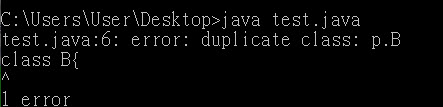
\includegraphics[width=75mm,scale=0.4]{SCN.jpg}}
\caption{\textbf{The error of using same class name for refactoring}}
\label{fig:renameclassname}
\end{figure}

Furthermore, this precondition is applicable to nested classes. The examples below show that we can not use the same name either as inner or as outer class for nested classes:

\begin{figure}[th]
\centering
\begin{minipage}[t]{0.75\linewidth}
\begin{lstlisting}[language=java, basicstyle=\scriptsize\ttfamily,frame=single]
package p;

public class A{	

  class M{
  }

  class N{
  }
} 
\end{lstlisting}
\end{minipage}
\caption{\textbf{Original Nested Class}}
\label{fig:original}
\end{figure}
\begin{itemize}
\item Example 1: The rename refactoring of the inner class can not be the same name as other inner classes' name. When we try to rename the inner class M to N as fig. \ref{fig:nestedclass1}, the java compiler shows up the error as fig. \ref{fig:NC1}.
\end{itemize}

\begin{figure}[th]
\centering
\begin{minipage}[t]{0.75\linewidth}
\begin{lstlisting}[language=java, basicstyle=\scriptsize\ttfamily,frame=single]
package p;

public class A{	
    
  class N{
  }
    
  class N{
  }
} 
\end{lstlisting}
\end{minipage}
\caption{\textbf{Example 1 of Nested Class Rename Refactoring}}
\label{fig:nestedclass1}
\end{figure}

\begin{figure}[H]
\centerline{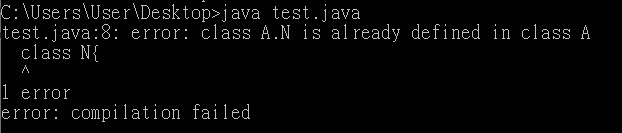
\includegraphics[width=75mm,scale=0.4]{NC1.jpg}}
\caption{\textbf{The error of duplicate inner class name for refactoring}}
\label{fig:NC1}
\end{figure}

\begin{itemize}
\item Example 2: The rename refactoring of the outer class can not be the same name as the inner classes' name, vice versa. When we try to either rename outer class to inner class name or rename inner class to outer class name, the java compiler shows up the error as fig. \ref{fig:NC2} and fig. \ref{fig:NC3}.
\end{itemize}

\begin{figure}[th]
\centering
\begin{minipage}[t]{0.45\linewidth}
\begin{lstlisting}[language=java, basicstyle=\scriptsize\ttfamily,frame=single]
package p;

public class M{	
  
  class M{
  }
	
  class N{
  }
} 
\end{lstlisting}
\tiny{(a) Rename Outer Class}
\end{minipage}
\hfill
\begin{minipage}[t]{0.45\linewidth}
\begin{lstlisting}[language=java, basicstyle=\scriptsize\ttfamily,frame=single]
package p;

public class A{	
    
  class A{
  }
    
  class N{
  }
} 
\end{lstlisting}
\tiny{(b) Rename Inner Class}
\end{minipage}
\caption{\textbf{Example 2 of Nested Class Rename Refactoring}}
\label{fig:nestedclass2}
\end{figure}

\begin{figure}[H]
\centerline{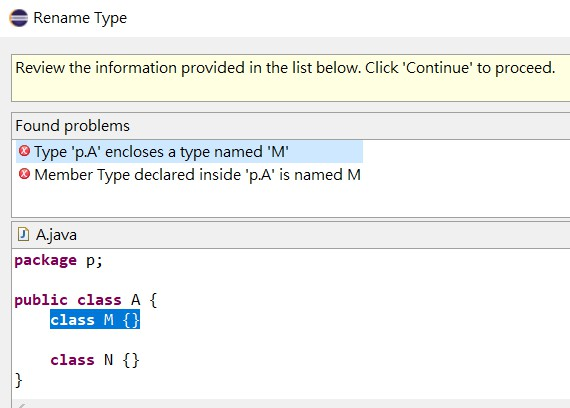
\includegraphics[width=75mm,scale=0.4]{NC2.jpg}}
\caption{\textbf{The error of renaming outer class as inner class name}}
\label{fig:NC2}
\end{figure}

\begin{figure}[H]
\centerline{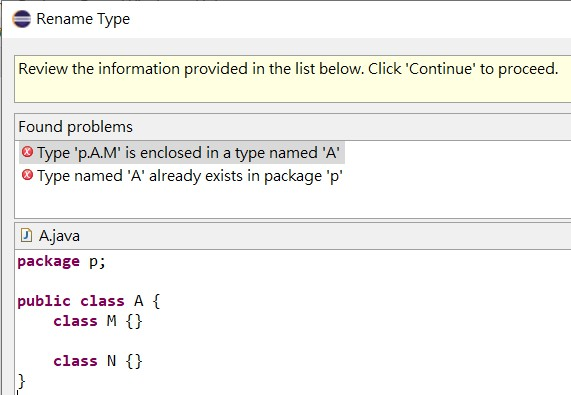
\includegraphics[width=75mm,scale=0.4]{NC3.jpg}}
\caption{\textbf{The error of renaming inner class as outer class name}}
\label{fig:NC3}
\end{figure}


Also, this precondition is applicable even if one or the other file is empty. So checking whether a class with the same name already exists in a package should be the first job we have to do for RcR. 
   
